
\hypertarget{menu_format}{}
\section{Format}
\index{format menu}

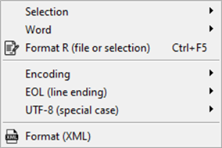
\includegraphics[scale=0.50]{./res/menu_format.png}\\

\begin{scriptsize}
  \begin{tabularx}{\textwidth}{>{\hsize=0.3\hsize}X>{\hsize=0.7\hsize}X}\\
    \hline
    \textbf{Option} & \textbf{Description} \\
    \hline
    Selection & \textit{\href{\#menu\_format\_selection}{See options ...}} \\
    Word & \textit{\href{\#menu\_format\_word}{See options ...}} \\
    Format R (file or selection) & Reformat a whole file or selection by using formatR package \\
    \hdashline[1pt/1pt]
    Encoding & \textit{\href{\#menu\_format\_encoding}{See options ...}} \\
    EOL (line ending) & \textit{\href{\#menu\_format\_eol}{See options ...}} \\
    UTF-8 (special case) & \textit{\href{\#menu\_format\_utf8}{See options ...}} \\
    \hdashline[1pt/1pt]
    Format (XML) & Formats XML files to be easily read by humans \\
    \hline
  \end{tabularx}
\end{scriptsize}


\hypertarget{menu_format_selection}{}
\subsection{Selection}
\index{format menu!selection}

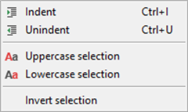
\includegraphics[scale=0.50]{./res/menu_format_selection.png}\\

\begin{scriptsize}
  \begin{tabularx}{\textwidth}{>{\hsize=0.4\hsize}X>{\hsize=0.6\hsize}X}\\
    \hline
    \textbf{Option} & \textbf{Description} \\
    \hline
    Indent & Indents selected line(s) \\
    Unindent & Unindents selected line(s) \\
    \hdashline[1pt/1pt]
    Uppercase selection & Converts selected text into upper case \\
    Lowercase selection & Converts selected text into lower case \\
    \hdashline[1pt/1pt]
    Invert selection & Inverts the case of all selected text \\
    \hline
  \end{tabularx}
\end{scriptsize}


\hypertarget{menu_format_word}{}
\subsection{Word}
\index{format menu!word}

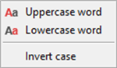
\includegraphics[scale=0.50]{./res/menu_format_word.png}\\

\begin{scriptsize}
  \begin{tabularx}{\textwidth}{>{\hsize=0.3\hsize}X>{\hsize=0.7\hsize}X}\\
    \hline
    \textbf{Option} & \textbf{Description} \\
    \hline
    Uppercase word & Converts the word under the cursor to upper case \\
    Lowercase word & Converts the word under the cursor to lower case \\
    \hdashline[1pt/1pt]
    Invert case & Inverts the case of the word under the cursor \\
    \hline
  \end{tabularx}
\end{scriptsize}


\newpage
\hypertarget{menu_format_encoding}{}
\subsection{Encoding}
\index{format menu!encoding}

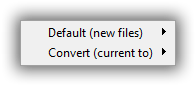
\includegraphics[scale=0.50]{./res/menu_format_encoding.png}\\

\begin{scriptsize}
  \begin{tabularx}{\textwidth}{>{\hsize=0.4\hsize}X>{\hsize=0.6\hsize}X}\\
    \hline
    \textbf{Option} & \textbf{Description} \\
    \hline
    Default (new files) & \textit{\href{\#menu\_format\_encoding\_default}{See options ...}} \\
    Convert (current to) & \textit{\href{\#menu\_format\_encoding\_convert}{See options ...}} \\
    \hline
  \end{tabularx}
\end{scriptsize}


\hypertarget{menu_format_encoding_default}{}
\subsubsection{Default (new files):}\\
\index{encoding}
\index{encoding!ANSI}
\index{encoding!UTF-8}
\index{encoding!UTF16-LE}
\index{encoding!UTF16-BE}

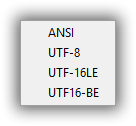
\includegraphics[scale=0.50]{./res/encoding.png}\\

\begin{scriptsize}
  \begin{tabularx}{\textwidth}{>{\hsize=0.3\hsize}X>{\hsize=0.7\hsize}X}\\
    \hline
    \textbf{Option} & \textbf{Description} \\
    \hline
    ANSI & Sets encoding to ANSI \\
    UTF-8 & Sets encoding to UTF-8 \\
    UTF16-LE & Sets encoding to UTF16-LE \\
    UTF16-BE & Sets encoding to UTF16-BE \\
    \hline
  \end{tabularx}
\end{scriptsize}


\hypertarget{menu_format_encoding_convert}{}
\subsubsection{Convert (current to):}\\

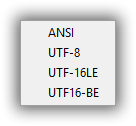
\includegraphics[scale=0.50]{./res/encoding.png}\\

\begin{scriptsize}
  \begin{tabularx}{\textwidth}{>{\hsize=0.3\hsize}X>{\hsize=0.7\hsize}X}\\
    \hline
    \textbf{Option} & \textbf{Description} \\
    \hline
    ANSI & Converts current encoding to ANSI \\
    UTF-8 & Converts current encoding to UTF-8 \\
    UTF16-LE & Converts current encoding to UTF16-LE \\
    UTF16-BE & Converts current encoding to UTF16-BE \\
    \hline
  \end{tabularx}
\end{scriptsize}


\hypertarget{menu_format_eol}{}
\subsection{EOL (line ending)}
\index{format menu!eol}

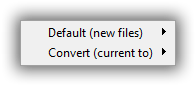
\includegraphics[scale=0.50]{./res/menu_format_eol.png}\\

\begin{scriptsize}
  \begin{tabularx}{\textwidth}{>{\hsize=0.4\hsize}X>{\hsize=0.6\hsize}X}\\
    \hline
    \textbf{Option} & \textbf{Description} \\
    \hline
    Default (new files) & \textit{\href{\#menu\_format\_eol\_default}{See options ...}} \\
    Convert (current to) & \textit{\href{\#menu\_format\_eol\_convert}{See options ...}} \\
    \hline
  \end{tabularx}
\end{scriptsize}


\newpage
\hypertarget{menu_format_eol_default}{}
\subsubsection{Default (new files):}\\
\index{EOL}
\index{EOL!WIN (CR+LF)}
\index{EOL!MAC (CR)}
\index{EOL!UNIX (LF)}

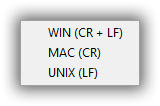
\includegraphics[scale=0.50]{./res/eol.png}\\

\begin{scriptsize}
  \begin{tabularx}{\textwidth}{>{\hsize=0.3\hsize}X>{\hsize=0.7\hsize}X}\\
    \hline
    \textbf{Option} & \textbf{Description} \\
    \hline
    WIN (CR+LF) & WIN (CR+LF) \\
    MAC (CR) & MAC (CR) \\
    UNIX (LF) & UNIX (LF) \\
    \hline
  \end{tabularx}
\end{scriptsize}


\hypertarget{menu_format_eol_convert}{}
\subsubsection{Convert (current to):}\\

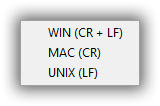
\includegraphics[scale=0.50]{./res/eol.png}\\

\begin{scriptsize}
  \begin{tabularx}{\textwidth}{>{\hsize=0.3\hsize}X>{\hsize=0.7\hsize}X}\\
    \hline
    \textbf{Option} & \textbf{Description} \\
    \hline
    WIN (CR+LF) & Convert to WIN (CR+LF) \\
    MAC (CR) & Convert to MAC (CR) \\
    UNIX (LF) & Convert to UNIX (LF) \\
    \hline
  \end{tabularx}
\end{scriptsize}


\hypertarget{menu_format_utf8}{}
\subsection{UTF-8 (special case)}
\index{format menu!UTF-8}

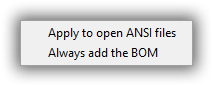
\includegraphics[scale=0.50]{./res/menu_format_utf8.png}\\

\begin{scriptsize}
  \begin{tabularx}{\textwidth}{>{\hsize=0.4\hsize}X>{\hsize=0.6\hsize}X}\\
    \hline
    \textbf{Option} & \textbf{Description} \\
    \hline
    Apply to open ANSI files & ANSI files without any special characters it will be always
      reconized as UTF-8 encoding \\
    Always add the BOM & When saving it will be always added the BOM \\
    \hline
  \end{tabularx}
\end{scriptsize}
